\subsection{Coin Flips}


\begin{lstlisting}
from sie import *
\end{lstlisting}

Generate a small list of data...

\begin{lstlisting}
data=randint(2,size=10)
print data
\end{lstlisting}

\begin{verbatim}
[1 0 0 1 0 0 0 1 0 0]
\end{verbatim}

Generate a slightly larger list of data...

\begin{lstlisting}
data=randint(2,size=30)
print data
\end{lstlisting}

\begin{verbatim}
[1 1 1 0 0 0 0 1 1 1 1 0 1 1 0 1 1 0 0 1 1 1 0 1 0 0 1 1 0 0]
\end{verbatim}

\begin{lstlisting}
data=randint(2,size=(2000,10))
data
\end{lstlisting}

\begin{verbatim}
array([[1, 0, 1, ..., 1, 0, 0],
       [1, 1, 1, ..., 0, 1, 0],
       [0, 0, 1, ..., 0, 0, 0],
       ..., 
       [0, 0, 0, ..., 1, 1, 0],
       [0, 1, 0, ..., 0, 1, 1],
       [0, 1, 1, ..., 1, 0, 1]])
\end{verbatim}

We have here a large collection of numbers (20000 of them!), organized in 2000
rows of 10 columns.  We can sum all of the 20000 values, or we can sum across
columns or across rows, depending on what we want.

\begin{lstlisting}
sum(data)  # add up all of the 1's
\end{lstlisting}

\begin{verbatim}
9988
\end{verbatim}

\begin{lstlisting}
sum(data,axis=0)  # sum up all of the columns
\end{lstlisting}

\begin{verbatim}
array([1011, 1010, 1001, 1051, 1001, 1008,  962,  990,  976,  978])
\end{verbatim}

\begin{lstlisting}
sum(data,axis=1)  # sum up all of the rows
\end{lstlisting}

\begin{verbatim}
array([3, 7, 3, ..., 5, 4, 6])
\end{verbatim}

Typically the hist command makes its own bins, which may not center on the
actual count values.  That's why we call countbins(N), to make bins centered on
the counts.

\begin{lstlisting}
N=sum(data,axis=1)  # number of heads in each of many flips
hist(N,countbins(10))
xlabel('Number of Heads')
ylabel('Number of Flips')
\end{lstlisting}

\begin{verbatim}
<matplotlib.text.Text at 0x10856e990>
\end{verbatim}

\begin{center}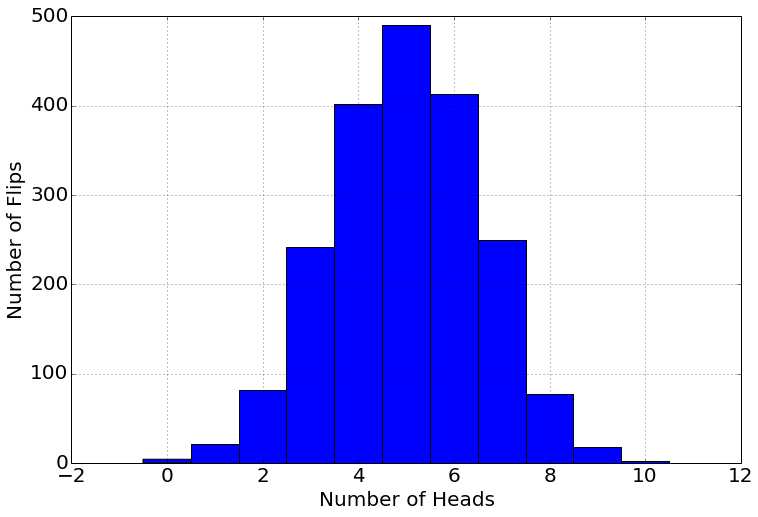
\includegraphics[width=4.5in]{Applications_of_Probability/Applications_of_Probability_fig0.png}\end{center}

To get a probability distribution, we divide the histogram result by $N$.

This distribution is Bernoulli's equation, or in other words, the binomial
distribution.

\[ p(h,10) = {10 \choose h} 0.5^h \cdot 0.5 ^{10-h} \]

\begin{lstlisting}
h=array([0,1,2,3,4,5,6,7,8,9,10])

# or...

h=arange(0,11)
\end{lstlisting}

(recall that ** is exponentiation in Python, because the caret (\^{}) was
already used for a computer-sciency role.)  The spaces in the equation below are
not needed, but highlight the three parts of the binomial distribution.

\begin{lstlisting}
p=nchoosek(10,h)* 0.5**h * 0.5**(10-h)
\end{lstlisting}

\begin{lstlisting}
hist(N,countbins(10),normed=True)
plot(h,p,'--o')
xlabel('Number of Heads, $h$')
ylabel('$p(h|N=10)$')
\end{lstlisting}

\begin{verbatim}
<matplotlib.text.Text at 0x108560290>
\end{verbatim}

\begin{center}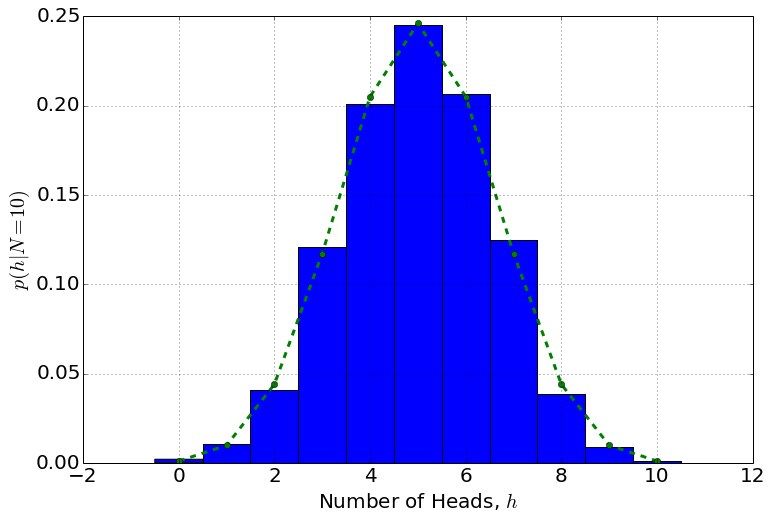
\includegraphics[width=4.5in]{Applications_of_Probability/Applications_of_Probability_fig1.png}\end{center}

